\documentclass[runningheads,a4paper]{llncs}
\usepackage{amssymb}
\setcounter{tocdepth}{3}
\usepackage{listings}
\usepackage{booktabs}
\usepackage{mathtools}
\usepackage{tabularx}
\usepackage{fixltx2e}
\PassOptionsToPackage{hyphens}{url}\usepackage{hyperref}
\usepackage[hyphens]{url}
\usepackage{upquote,textcomp}
\lstset{breaklines=true, basicstyle=\scriptsize\ttfamily, upquote=true}

\usepackage{fancyvrb}
\VerbatimFootnotes
\usepackage{cprotect}

\usepackage{graphicx}
\makeatletter
\def\maxwidth#1{\ifdim\Gin@nat@width>#1 #1\else\Gin@nat@width\fi}
\makeatother

\usepackage{amsmath}
\usepackage{pmml-new}

\usepackage{color,graphics,array,csscolor}

\usepackage{fontspec,unicode-math}
\usepackage[Latin,Greek]{ucharclasses}
\setTransitionsForGreek{\fontspec{Times New Roman}}{}

\usepackage{subscript}
\lstset{breaklines=true, basicstyle=\scriptsize\ttfamily}

\begin{document}
\mainmatter

\title{PRESS: A Publication REpository Semantic System}
\titlerunning{PRESS}
\author{Ioannis Chrysakis\inst{1} \and
Emmanouil Dermitzakis\inst{1} \and
Giorgos Flouris\inst{1} \and
Theodore Patkos\inst{1} \and
Dimitris Plexousakis\inst{1}}
\authorrunning{Ioannis Chrysakis et al.}
\institute{Foundation for Research and Technology Hellas, Institute of Computer Science\\
\email{hrysakis@ics.forth.gr, 
dermitz@ics.forth.gr, 
fgeo@ics.forth.gr, 
patkos@ics.forth.gr, 
dp@ics.forth.gr}}
\maketitle

\begin{abstract}
Publication management systems can be instrumental in disseminating research results across academia and industry, by providing facilities for uploading, editing and searching for publications. Usually, these systems can be used by individuals to assist them in their research or by organizations to help them classify and promote their publication items. In this paper, we present PRESS, an open-source publication system that exploits semantic technologies in order to cover the needs of both individuals and organizations. Thus, it supports fast data entry, advanced query capabilities and integration with other systems or datasets.

\keywords{digital libraries, linked data, ontology management, publication systems, web semantics}
\end{abstract}


\section{Introduction}

Technological and science evolution frequently leads to innovative research results that can be exploited to improve our life through new techniques, products and services. Typically, research results are recorded in publications in order to keep academia and industry always informed. Thus, scientists and developers can be assisted to extend and evolve their work or to be inspired towards new discoveries. Moreover, inside a lab or a large organization there is a need to store publications into an open repository, which should be easily accessible to the public for the purposes of dissemination, or for reasons related to internal document classification. In fact, we can find systems that automatically aggregate or index publications like Google Scholar and DBLP. 

Therefore, it is valuable to deploy systems that can store and organize the different types of publications for easy browsing and exploration. This is the aim of publication management systems, which provide facilities for both ingestion and searching in a corpus of publications. Although a variety of commercial systems exists, this paper provides an advanced, open-source solution, which facilitates flexible customization, independence and integration. Most other open-source approaches offer limited search capabilities, because they rely on rigid relational schemes and could not exploit semantics.

We employ semantic technologies to provide more advanced search capabilities and full classification of publications on a system that follows a loosely-coupled architecture. More precisely, we use a custom ontology that covers the proposed classification scheme and is compatible with the CERIF model  \cite{_Ref474417470} a standard that the EU recommends to its member states for recording information about research activity. To validate our approach, we load a dataset to the repository that contains actual publications and has been originally expressed in CERIF XML format.



\section{Related Work}

Publication systems are part of the wider class of integrated library systems (ILS). Focusing on those that provide functionalities for both inserting and searching for publications we can distinguish between commercial and open-source solutions. 

Commercial solutions are designed mainly for expert users, such as librarians, and offer automation on traditional librarian tasks, such as digitizing, cataloguing and storing publications. The Ex Libris by ProQuest\footnote{ http://www.exlibrisgroup.com/} has gained status as the largest technology provider to academic libraries  \cite{_Ref490663034} offering APIs, platforms and discovery services. Similarly OCLC\footnote{ https://www.oclc.org/} and Bibliotheca\footnote{ http://www.bibliotheca.com} provide a variety of commercial apps (i.e. cloudLibrary, Worldshare Management Services) that can satisfy the end user in terms of ingesting or browsing publication content. Although these solutions are robust, they are not public and extensible (some of them do not even provide a web interface), and cannot address specialized needs. 

Open-source solutions include Dspace\footnote{ http://www.dspace.org/}, Koha\footnote{ http://www.koha.org/} and Fedora\footnote{ https://getfedora.org/}. Dspace and Koha have the advantage of providing a web interface, which facilitates the use of a typical publication system by academic or research institutes.  Fedora is an open source repository system, but lacks an interface for the related features. The main limitation of these systems is their difficulty in expressing complex queries beyond the typical text search as this presupposed knowledge of the underlying relational database schemas. Another approach is to employ a content management system (CMS), like Drupal, and its supported publications modules (e.g. Biblio). The limitation of this solution is that the system can become so bound to the CMS and to its respective relational database, thereby reducing query capabilities. Bibbase\footnote{ https://bibbase.org/} dynamically renders an up-to-date HTML page enabling a web based solution with easy setup and integration, based on bib files which are processed centrally by the BibBase server.

OpenAIRE\footnote{ https://www.openaire.eu/}  is a participatory European open access infrastructure that acts as aggregator of scientific publications and associated material via repository networks like Zenodo\footnote{ https://www.zenodo.org/}. It does not actually stores publications but exposes them using Dublin Core model\footnote{ http://dublincore.org/} through respective LOD services, while offering guidelines to support CERIF-XML semantics. Finally, Folio\footnote{  https://www.folio.org/platform/} is a recent community-based approach that represents a partnership between libraries and vendors aiming to create an open source library services platform and a "plug-and-play" application that will function as a cohesive experience in a single user interface.

\section{Methodology}

\subsection{Semantics}

Semantic Web technology enables more sophisticated knowledge management, by applying evolving and refactoring schemas, metadata and relationships between them  \cite{_Ref490663279}. The flexibility of semantically enriched data gives rise to the implementation of efficient semantics-aware applications that can facilitate data integration, support knowledge enrichment and advanced query capabilities by searching between multiple patterns across the metadata. 

Our system leverages such technologies by developing a basic ontology in OWL (called Press Ontology) which is CERIF compatible and captures the core schema containing basic entities that are related with each publication, and their respective properties and relationships. The ontology (see Fig.~\ref{_Ref490663813}) consists of 6 top classes, 4 main (Publication, Person, Laboratory and Project) and 2 complementary ones (List, List\_Slot). The latter are used for keeping the sequence on items following the approach of  \cite{_Ref490663486}. Classes are connected through 7 object properties that denote their relationships. We use 47 data properties to cover all attributes of a publication.  
\begin{figure}[h!]
\centering
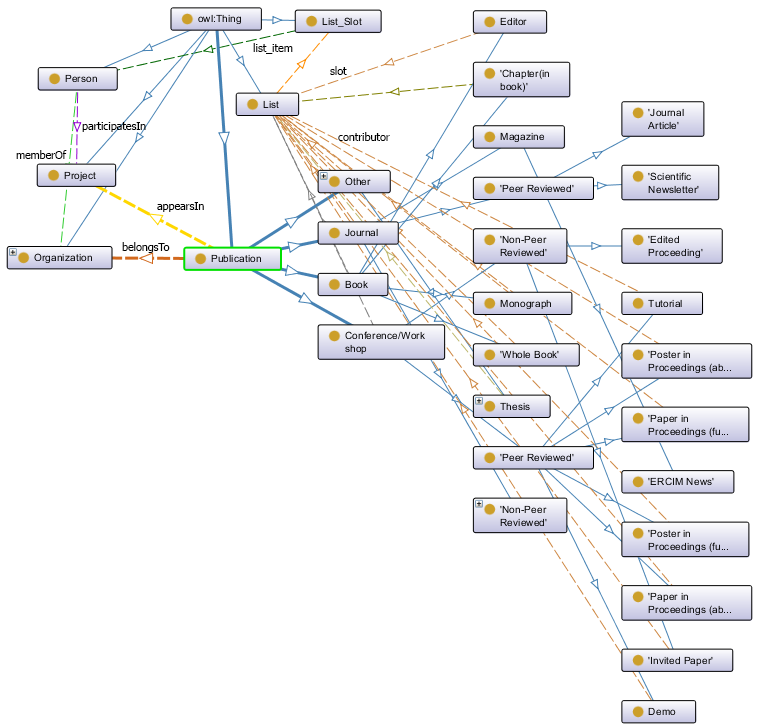
\includegraphics[width=\maxwidth{\textwidth}]{./img/image1.png}
\cprotect\caption{The PRESS Ontology}
\label{_Ref490663813}
\end{figure}


The Publication class contains 4 direct subclasses and various indirect ones, representing different publication types (e.g., Book, Conference/Workshop etc). Different properties are used to connect publications to their authors (a property to the Person Class), authors' affiliations (property to Organization) and projects that funded the work (property to Project Class). We use the FOAF ontology\footnote{ http://xmlns.com/foaf/spec/} for Person entities. Finally, the PRESS ontology provides features like keeping the order of authors, distinguishing peer reviewed from non-peer reviewed publications, better query evaluation based on indirect classes classification and a small but comprehensive schema. For each publication we store metadata information as RDF triples to the Blazegraph\footnote{ https://www.blazegraph.com/} repository which is an ultra-scalable, open-sourced, high-performance graph database which can store up to 50B triples/quads. It is a plug and play cross-platform software, which also provides a REST API with an embedded endpoint for enabling SPARQL query functionalities. 

\subsection{Architecture}

For the basic functionalities of PRESS we chose Drupal\footnote{ https://www.drupal.org/}, a robust CMS with a large established community that enables scalable development of web modules. PRESS can be conceptually divided into four main groups for the installed modules plus one for our developed module (see Fig.~\ref{_Ref490664034}). All modules communicate with each other independently of their conceptual group since they are built with the same Web Programming technologies. The first group deals with the {\em User Authentication }containing modules for leveraging security to the system. The second group ({\em UI Modules}) is related with modules necessary for the User Interface development. The third group consists of {\em Back-End modules} which are necessary for the unique identification and storing of each publication, enabling search engine optimization and sharing of external libraries. The core drupal functionalities are provided by the default {\em Core Modules }group.  Finally, the drupal module that we implemented (named {\em Publication Module}) creates one page per publication, and displays all the relevant information that can be edited later by each author.
\begin{figure}[h!]
\centering

\includegraphics[width=\maxwidth{\textwidth}]{./img/image2.png}
\cprotect\caption{The PRESS Architecture}
\label{_Ref490664034}
\end{figure}


Also, we developed a library ({\em PRESS library}) that deals with the basic user interfaces for inserting, editing or searching for any publication exploiting the core UI modules and the publication module. Finally, the actual document of publication is stored as a pdf file in the file system of the webserver, exploiting the core modules of Drupal. Our architecture is loosely-coupled. Thus, we can replace existing modules (e.g., user authentication), interfaces (e.g. search interface), or even the ontology schema with alternative implementations without jeopardizing data consistency. All data is accessible through a public SPARQL endpoint. 

\subsection{Features and Innovation}

The core innovative feature of PRESS is its advanced query capabilities. For example, it supports full free text queries by using the extended RDF predicate {\em bds:search} of SPARQL, as it has been implemented in Blazegraph. Moreover, with SPARQL, we can make complex and expressive queries upon RDF/OWL metadata, such as cross snapshot queries, range queries on dates etc.  The use of Blazegraph Repository ensures scalability and stability  \cite{_Ref490664453} for the storing of all semantic information. Another advantage of PRESS is that it is open-source, cross platform, web-based and requires low resources to run  \cite{_Ref490664467}. It is extensible and currently integrated with Drupal CMS. In addition, a core design decision was for the system to be usable by all kinds of users, and not just experienced ones (i.e. librarians). Towards this end, we support a responsive and user-friendly interface, a basic security policy, import/export facilities (using DOI) and search engine optimization techniques. To the best of our knowledge there is no other semantic-aware open-source publication system that can provide all the above functionalities.

\section{Implementation}

\subsection{The Press System}

We will now present briefly two basic user interfaces of PRESS that implemented using the bootstrap library\footnote{ http://getbootstrap.com/}. The authenticated user has two options: to add a publication manually via a webform, or to enter the respective DOI  \cite{_Ref490665523} (see Fig.~\ref{_Ref490666384}). In the first option the user has to select a category and a subcategory and in turn to fill in the dynamic fields of the form. The second option helps users to automatically fill in all the fields by extracting information of the imported DOI embedding the CrossrefOpen URL resolver functionality. PRESS can automatically add an author, which is authorized (via LDAP module) or can manually add a new one. Also, it can change the order via drag and drop functionality. Furthermore, user-defined tags could be added per publication for extra classification purposes.

The search interface gives three options of searching (see Fig.~\ref{_Ref490666406}): full-text search, advanced search and browsing by category. The full text search capability provides fast retrieving information of a keyword or a phrase that is contained in at least one attribute of a publication. The advanced search offers query templates that can be enabled dynamically according to user options and under specified concepts (i.e peer reviewed publications). These templates can be configured to support any kind of linked concept (semantically any class or property). Finally, the browsing by category gives a supervisory look of the current status of the publication repository focusing on the classification of the publications. In each top category the user can browse the related articles by clicking on the name of the category or open up the dynamic panel for more specific categories.
\begin{figure}[h!]
\centering
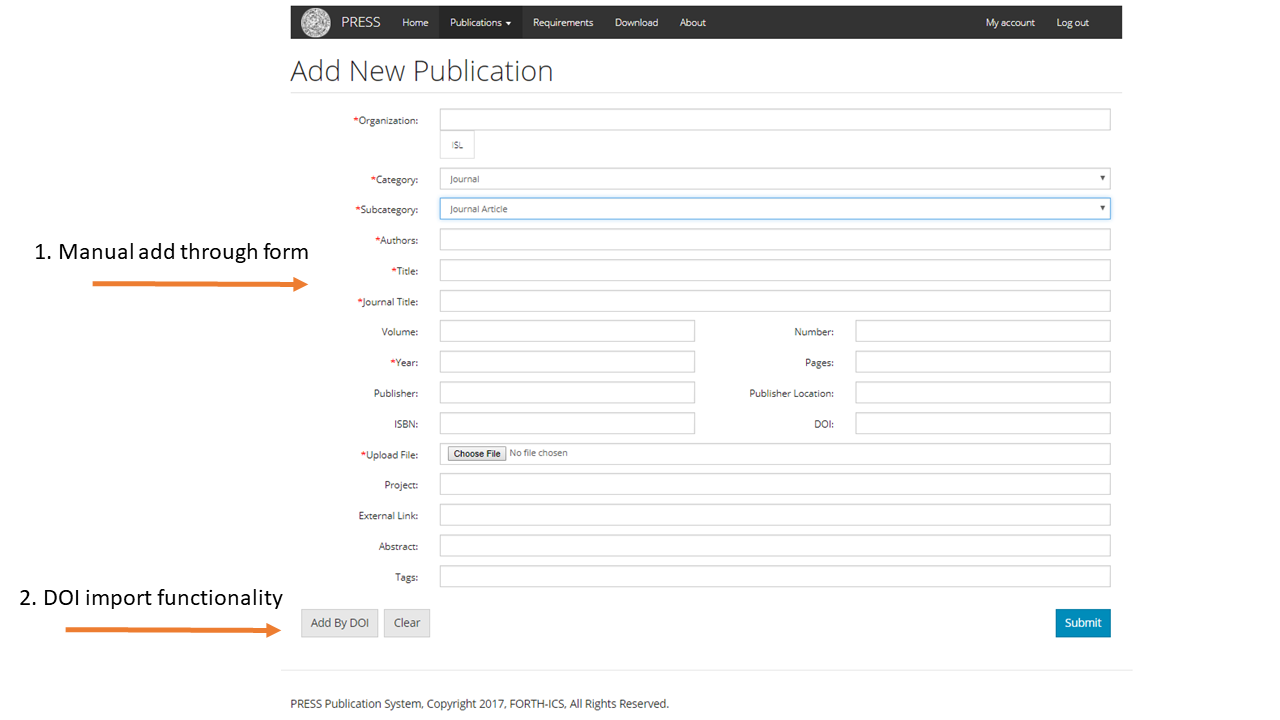
\includegraphics[width=\maxwidth{\textwidth}]{./img/image3.PNG}
\cprotect\caption{The Add UI}
\label{_Ref490666384}
\end{figure}

\begin{figure}[h!]
\centering
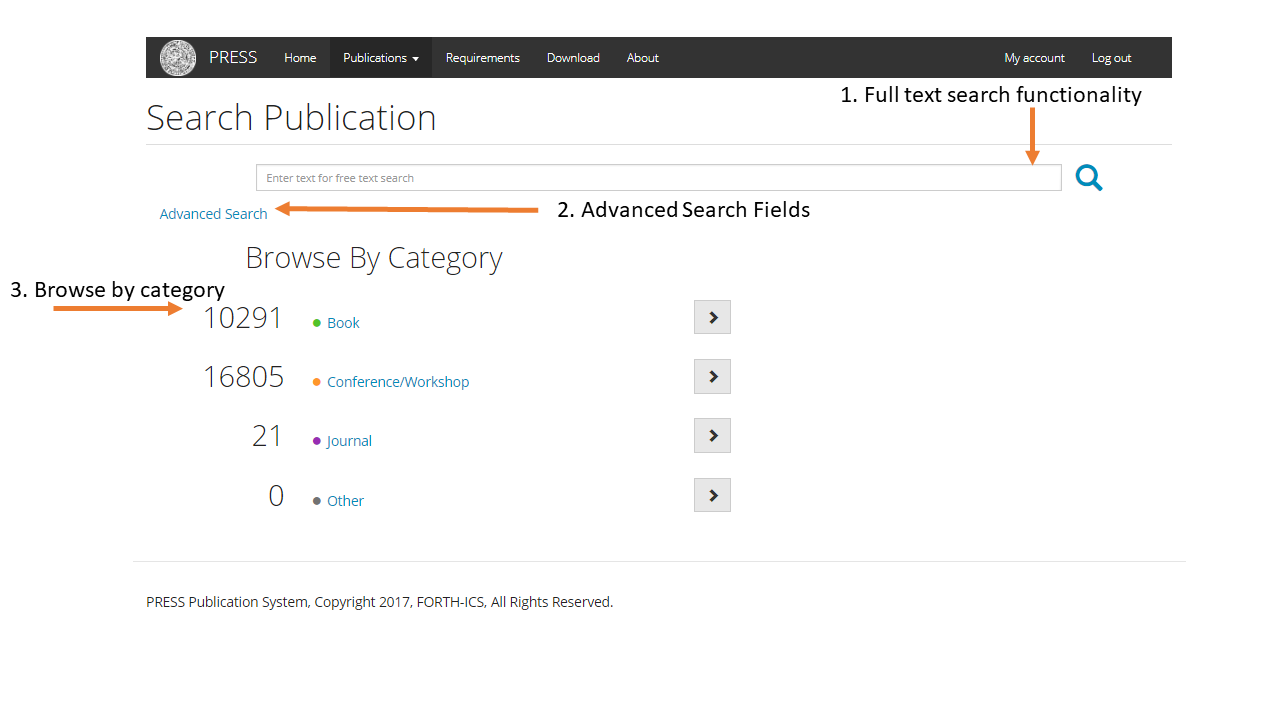
\includegraphics[width=\maxwidth{\textwidth}]{./img/image4.PNG}
\cprotect\caption{The Search UI}
\label{_Ref490666406}
\end{figure}


\subsection{Use Case -- The VRE4EIC Project}

The VRE4EIC is an ongoing EU project that aims at providing a Europe-wide interoperable Virtual Research Environment (VRE) to empower multidisciplinary research communities. The project will result in a reference architecture for VREs, along with software components that exploit metadata from publications, persons, organizations and projects following the CERIF model. We used the 3M tool  \cite{_Ref490665546} to create the appropriate mappings, in order to align our ontology schema and to make the data fully compatible with the project's approach. For demonstration purposes, we further loaded the synthetic datasets of publications that come from EKT repository referring to 1.76M Triples and finally deployed an installation of PRESS  \cite{_Ref490664467}. This use case shows in practice that the system can be simply adapted to the different needs of research institutes and can be scalable enough with semantic linked data that are located in the semantic repository.

\section{Future Work}

We are currently working on improving user's search and import experience by adding some extra features to PRESS like providing more elaborate statistics per year, author, project etc. Finally, our desire is to support more import and export utilities by exploiting bib files. 

\subsubsection*{Acknowledgements.}This work has been partially funded from the EU H2020 VRE4EIC project under grant agreement No. 676247.


\begin{thebibliography}{4}

\bibitem{_Ref490664453} \url{https://utecht.github.io/rdf/triple\%20stores/comparing-triplestores/}
\bibitem{_Ref490663034} Library Systems Report (2017). American Libraries Magazine. 1 May, 2017. \url{https://americanlibrariesmagazine.org/2017/05/01/library-systems-report-2017/}
\bibitem{_Ref490665546} Marketakis, Y., Minadakis, N., Kondylakis, H., Konsolaki, K., Samaritakis, G., Theodoridou, M., Flouris, G., \& Doerr, M. (2016). X3ML Mapping Framework for Information Integration in Cultural Heritage and Beyond. International Journal on Digital Libraries, Special Issue on ``Extending, Mapping and Focusing the CIDOC CRM'', 1-19.
\bibitem{_Ref474417470} The CERIF Model:\url{http://www.eurocris.org/cerif/main-features-cerif}
\bibitem{_Ref490665523} The DOI Handbook:\url{https://www.doi.org/hb.html}
\bibitem{_Ref490663486} The Ordered List Ontology: \url{http://smiy.sourceforge.net/olo/spec/orderedlistontology.html}
\bibitem{_Ref490664467} The PRESS demo:\url{https://www.ics.forth.gr/isl/PressDemo}
\bibitem{_Ref490663279} Tim Berners-Lee, James Hendler \& Ora Lassila (2001): The Semantic Web: A new form of Web content that is meaningful to computers would unleash a revolution of new possibilities, Scientific American.

\end{thebibliography}

\end{document}